\documentclass[11pt,fleqn]{article}

\setlength {\topmargin} {-.15in}
\setlength {\textheight} {8.6in}

\usepackage{amsmath}
\usepackage{amssymb}
\usepackage{color}
\usepackage{tikz}
\usetikzlibrary{automata,positioning,arrows}
\usepackage{diagbox}
\usepackage{stackrel}

\newcommand{\be}{\begin{enumerate}}
\newcommand{\ee}{\end{enumerate}}

\begin{document}
\textbf{Exercise 4.2.43 Reachable Vertex in Digraph:} Design a linear-time algorithm to determine whether a digraph has a vertex that is reachable from every other vertex\\

\textbf{Solution:} If a vertex is reachable from every other vertex in digraph, then it must be last strong component of the digraph assuming topological order. Recall the last node in topological order is known as sink known while beginning node is called source node. The sink node has zero out-order because no arrows come out of it to point to other nodes. Arrows only go into to as other nodes point to this node as it is the last node.\\

Recall a digraph has a topological order iff it is a DAG(Directed Acyclic Graph) which is a graph with no cycles. A cut of a graph is partition of vertices in 2 non-empty sets. A crossing edge of a cut is an edge that connects a vertex in one set with a vertex in another. The crossing edge of min weight graph is MST(Min spanning tree) of graph.

\be
	\item Compute SCC using Kosaraju-Sharirs Algorithm which uses 2 DFS instances.
	\item This means the first node in SCC is actually last node of topological order
	\item 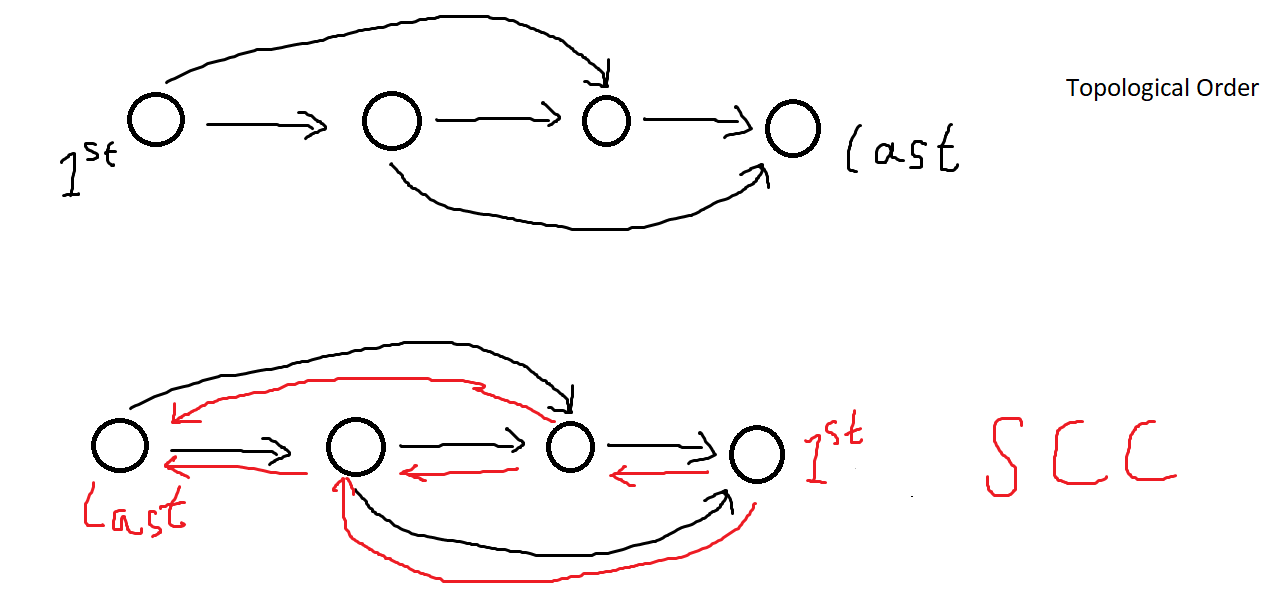
\includegraphics[scale=0.4]{4.2.43.png}
	\item Do DFS from first vertex in last strong component on Reverse Topological Order(TO) shown in red above.
	\item If all vertices visited from this vertex, then this vertex is reachable from every other vertex as it is correctly reached by every vertex when it was previously the sink node, and now it can reach every other vertex as the source node.
\ee

\newpage

Summary of what we did on previous page:\\
There is always some set of SCCs with 0-outdegree. Calling DFS on any node in a 0-SCC finds nodes in that 0-SCC. Recall Topological orders can have cycles. So the TO in the previous page had nodes which were actually cluster of many nodes OR the nodes themselves were SCCs to avoid cycles.\\

For topological order, there must be a source and end node. The end node is reachable from all other nodes and has zero out-order as described on previous page.\\

We can verify this and have done so by traversing back from sink to source using DFS to see if a source exists. If it does, then the TO is valid and so is the SCC diagrams.



\end{document}
